\chapter*{La Paz, Huayna Potosi et route de la mort\markboth{La Paz, Huayna Potosi et route de la mort}{}}
\section*{11 mai 2015}

À La Paz je suis hébergé à la Casa de Ciclistas, une maison qui accueille tous les cyclistes de passage, on était entre 5 et 10 personnes en permanence. J'y retrouve Lucie et Frédéric ainsi que Tim, un anglais déjà croisé dans le Sud Lipez. La ville est tout en dénivelé, plus de 400m entre El Alto et le centre de La Paz à 3600m.

Vue depuis le parc Laikakota. 
\begin{center} 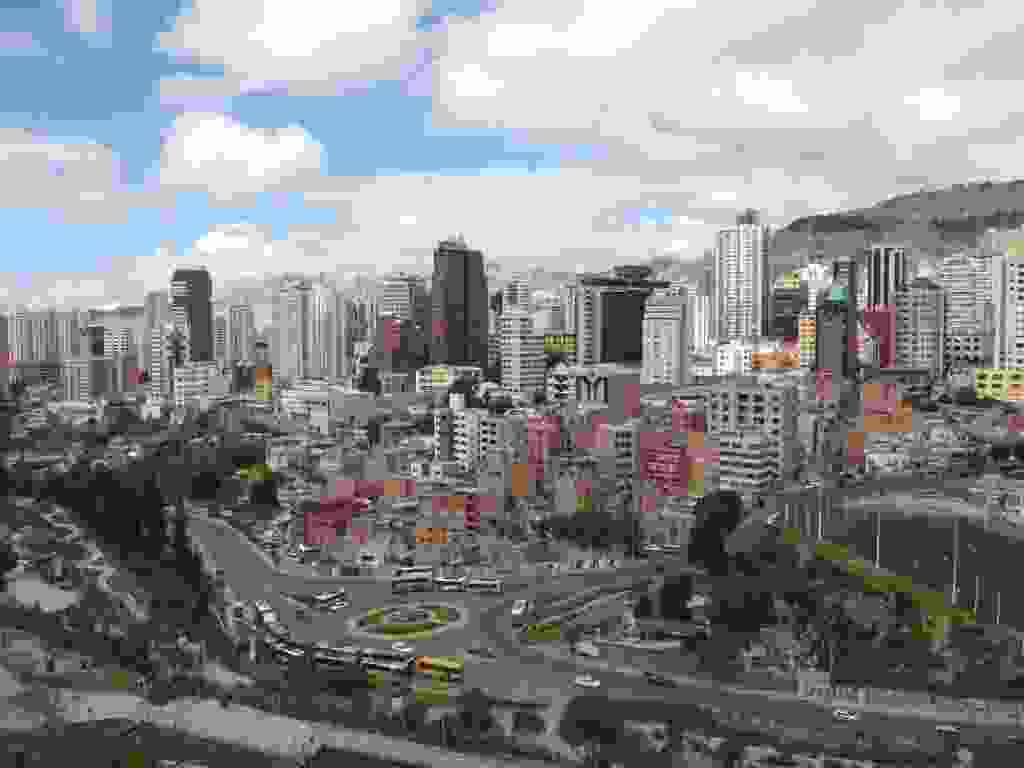
\includegraphics[width=\mywidth]{../wp-content/uploads/2015/05/P4293689-1024x768.jpg} \end{center}
\begin{center} 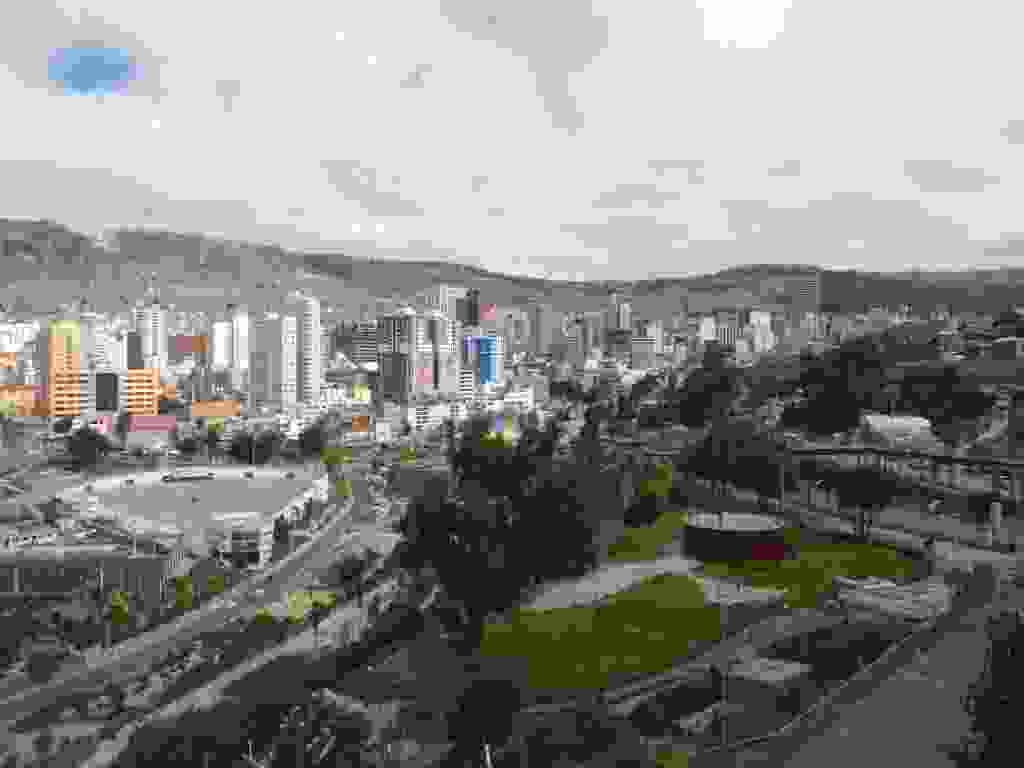
\includegraphics[width=\mywidth]{../wp-content/uploads/2015/05/P4293691-1024x768.jpg} \end{center}

Vue depuis le mirador Killi Killi. 
\begin{center} 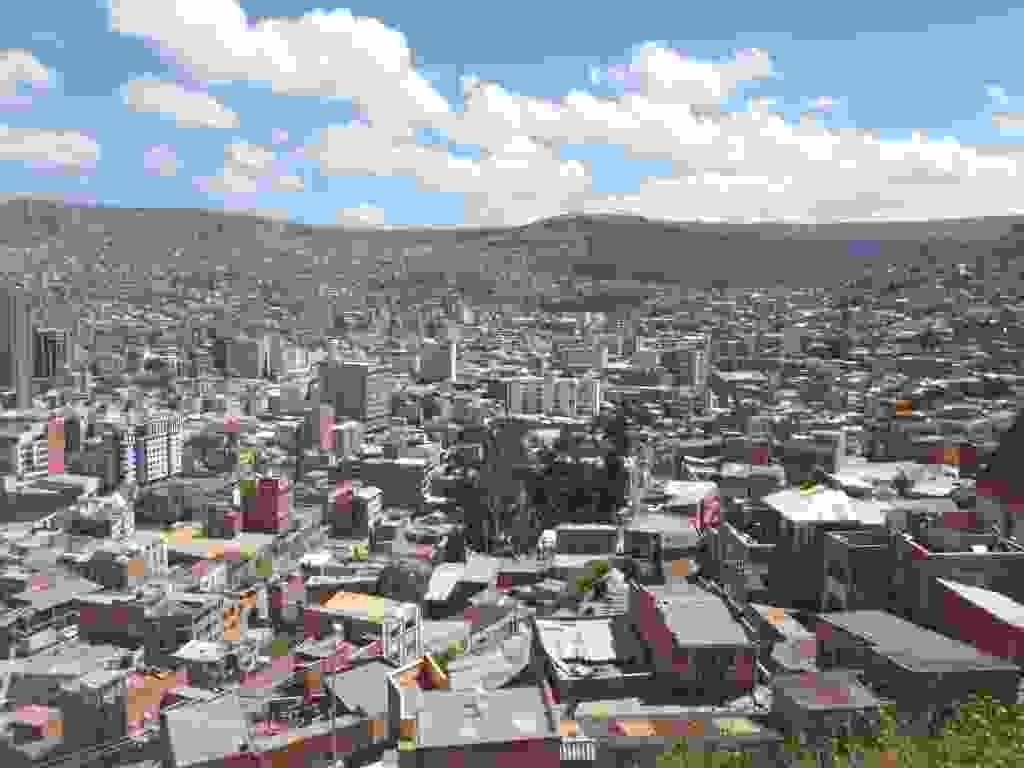
\includegraphics[width=\mywidth]{../wp-content/uploads/2015/05/P4293699-1024x768.jpg} \end{center}
\pagebreak

La Plaza Murillo avec la cathédrale et le palais gouvernemental. 
\begin{center} 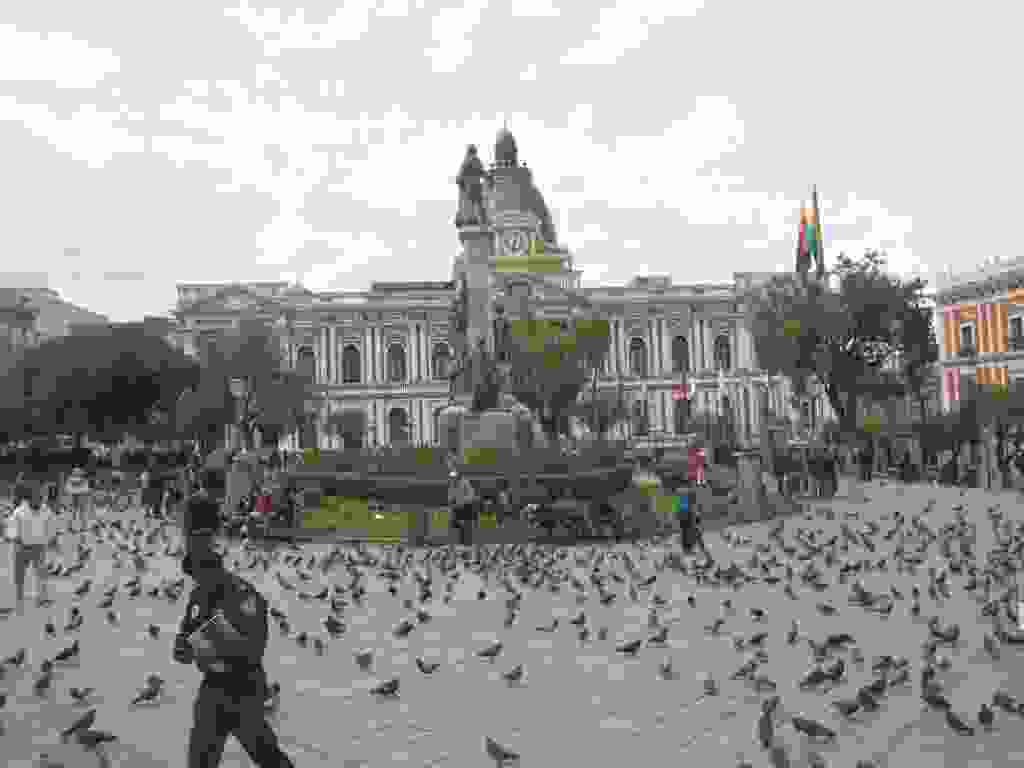
\includegraphics[width=\mywidth]{../wp-content/uploads/2015/05/wpid-wp-1430959404815-1024x768.jpg} \end{center}
\begin{center} 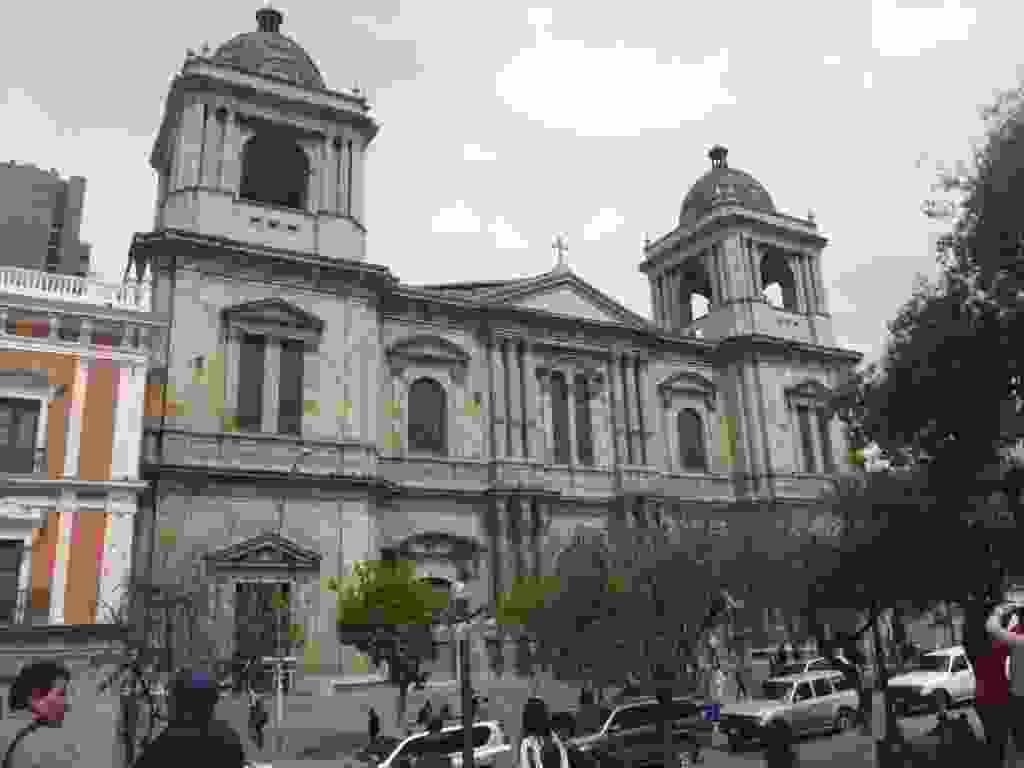
\includegraphics[width=\mywidth]{../wp-content/uploads/2015/05/P4283684-1024x768.jpg} \end{center}
\pagebreak

L'église San Francisco. 
\begin{center} 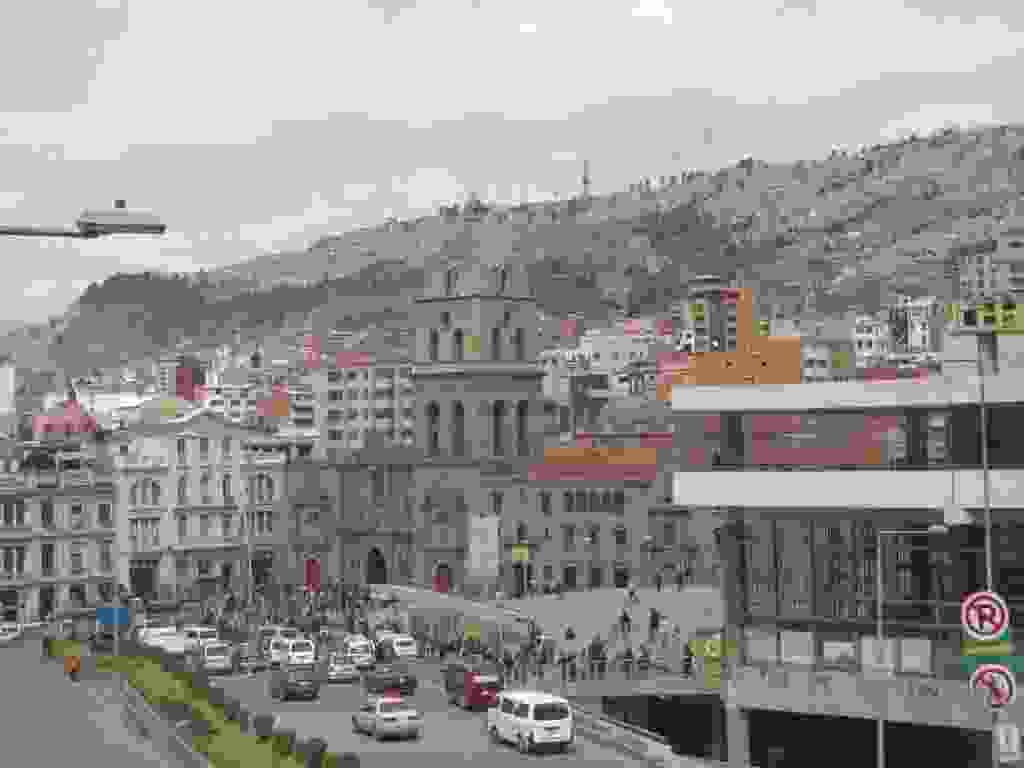
\includegraphics[width=\mywidth]{../wp-content/uploads/2015/05/P4283680-1024x768.jpg} \end{center}

Je suis allé faire l'ascension du Huayna Potosi à quelques dizaines de km de La Paz. 
\begin{center} 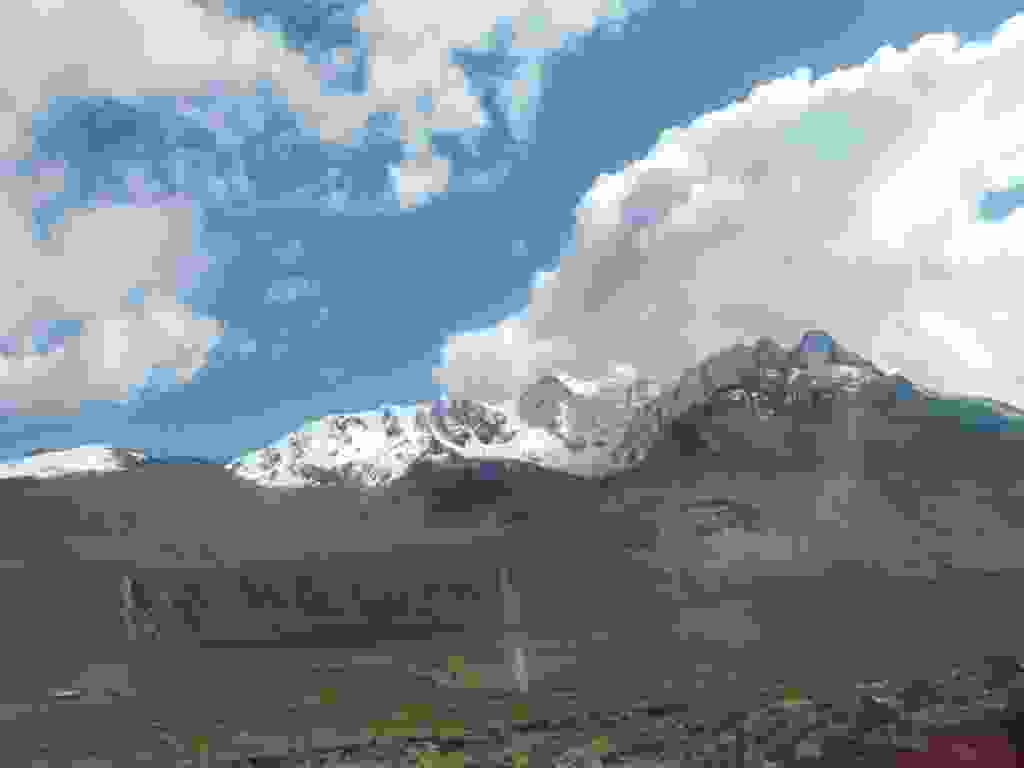
\includegraphics[width=\mywidth]{../wp-content/uploads/2015/05/P4303702-1024x768.jpg} \end{center}
\pagebreak

Premier jour montée au glacier pour s'exercer aux crampons/piolet. Je suis avec Fernando, brésilien et notre guide Santos. 
\begin{center} 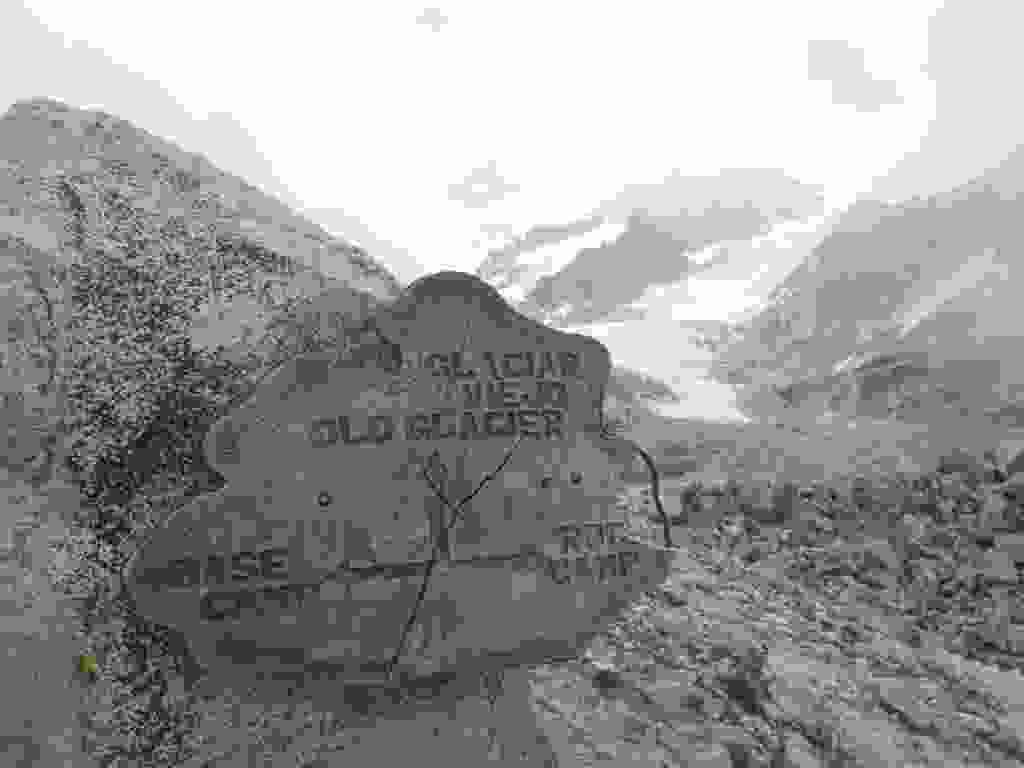
\includegraphics[width=\mywidth]{../wp-content/uploads/2015/05/P4303705-1024x768.jpg} \end{center}
\begin{center} 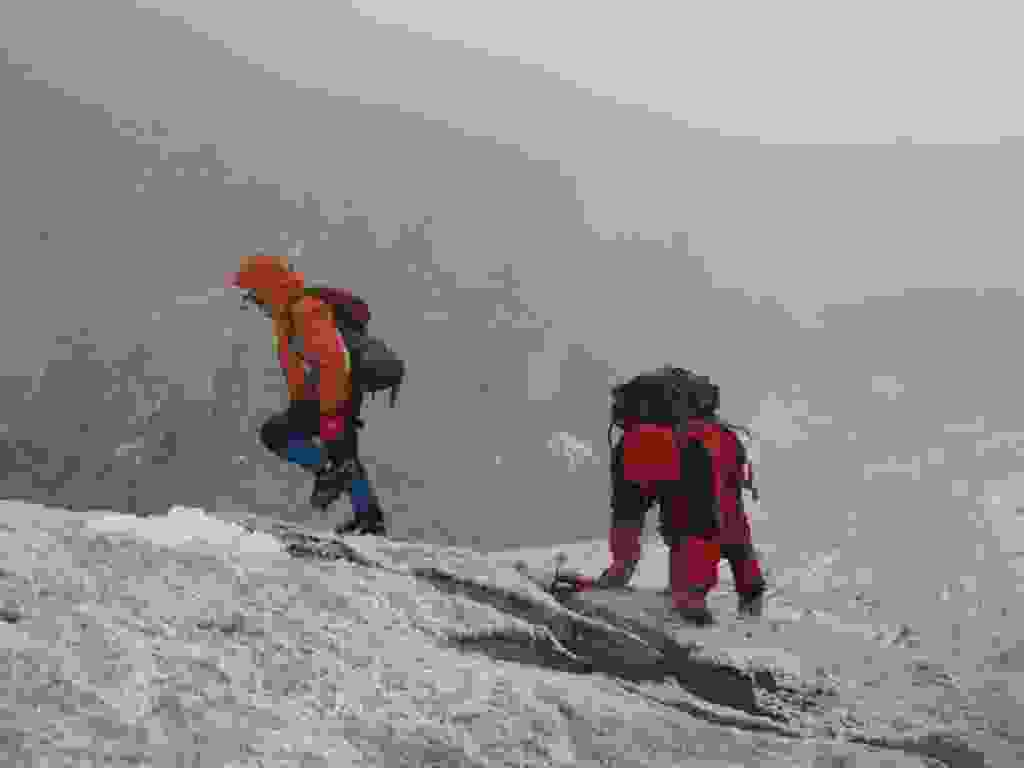
\includegraphics[width=\mywidth]{../wp-content/uploads/2015/05/P4303707-1024x768.jpg} \end{center}

\begin{center} 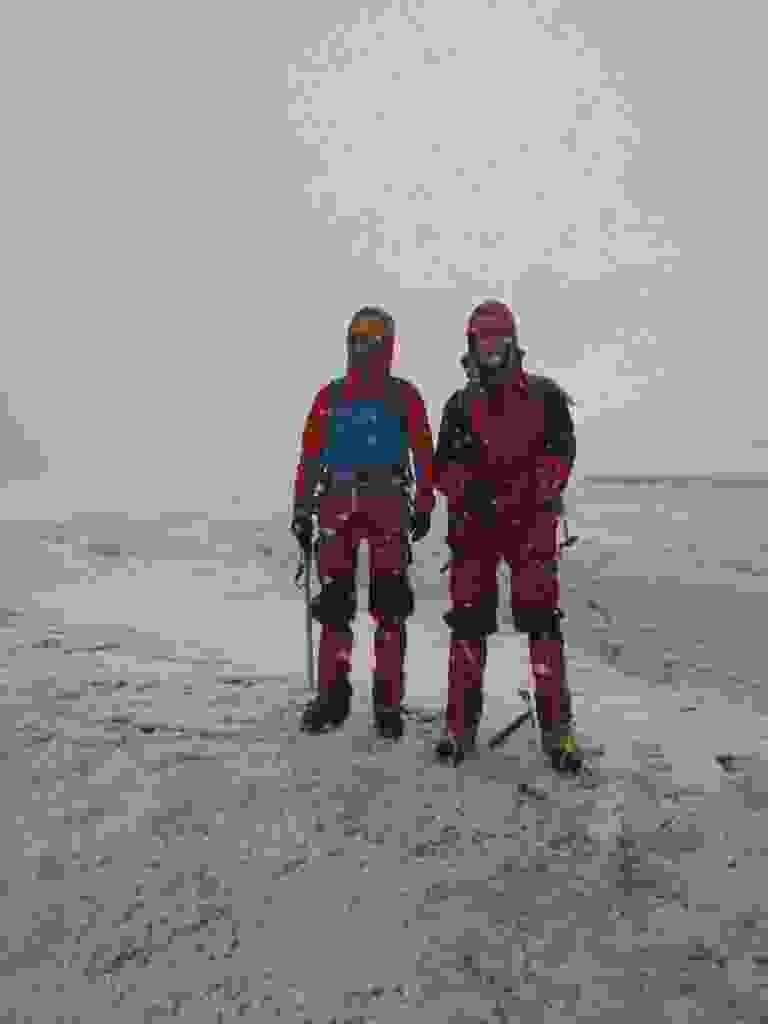
\includegraphics[width=0.6\textwidth]{../wp-content/uploads/2015/05/P4303710-768x1024.jpg} \end{center}

Retour au camp de base pour la nuit. 
\begin{center} 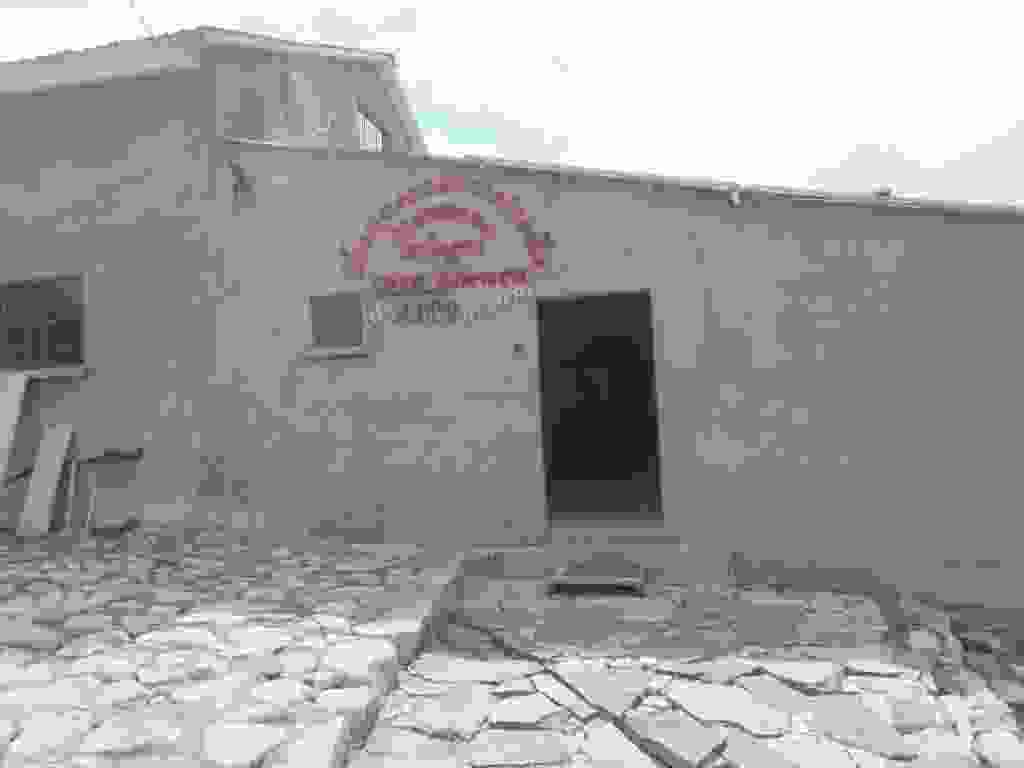
\includegraphics[width=\mywidth]{../wp-content/uploads/2015/05/P4303704-1024x768.jpg} \end{center}
\pagebreak

Montée au camp d'altitude le deuxième jour. 
\begin{center} 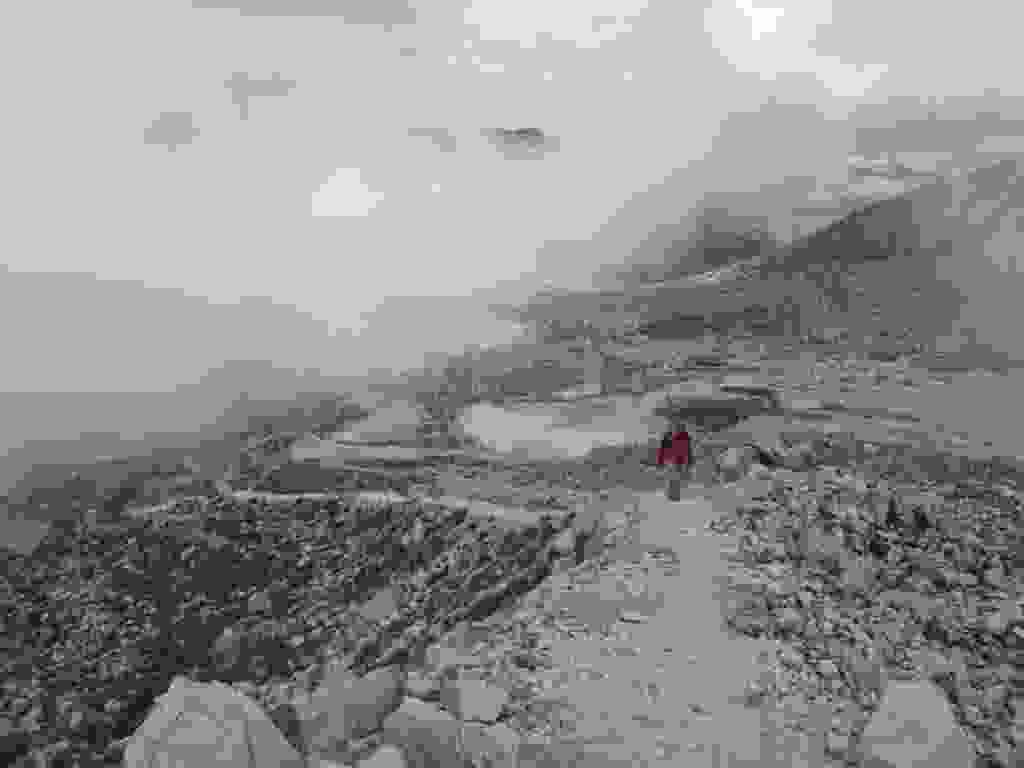
\includegraphics[width=\mywidth]{../wp-content/uploads/2015/05/P5013714-1024x768.jpg} \end{center}
\begin{center} 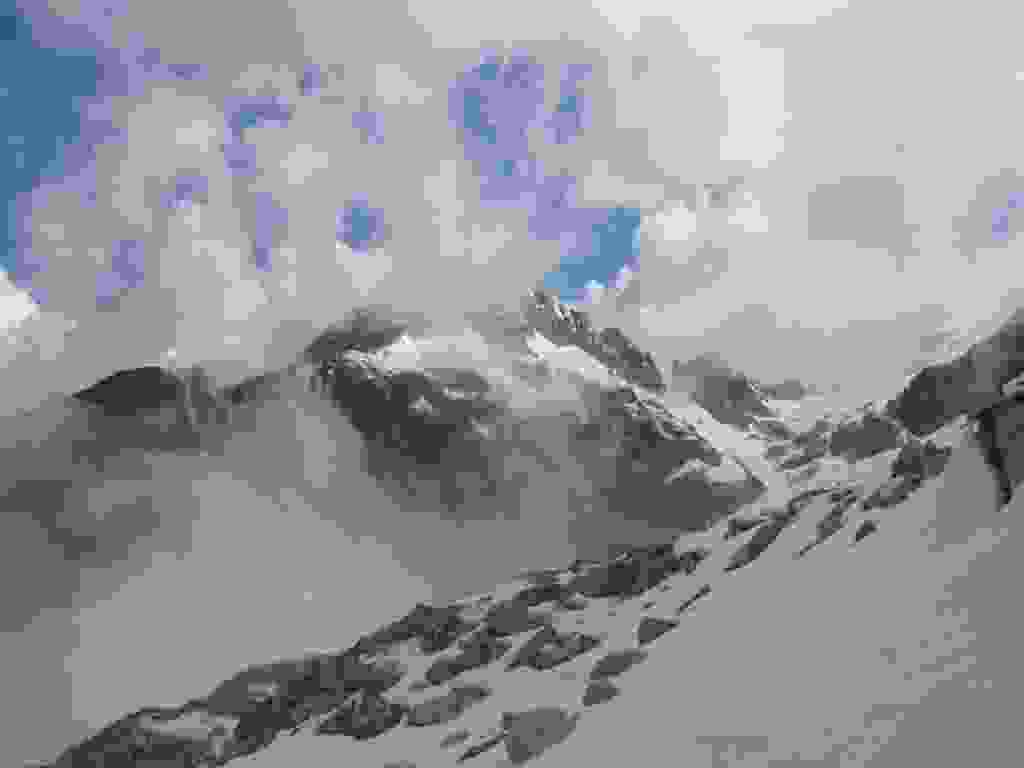
\includegraphics[width=\mywidth]{../wp-content/uploads/2015/05/P5013725-1024x768.jpg} \end{center}

\begin{center} 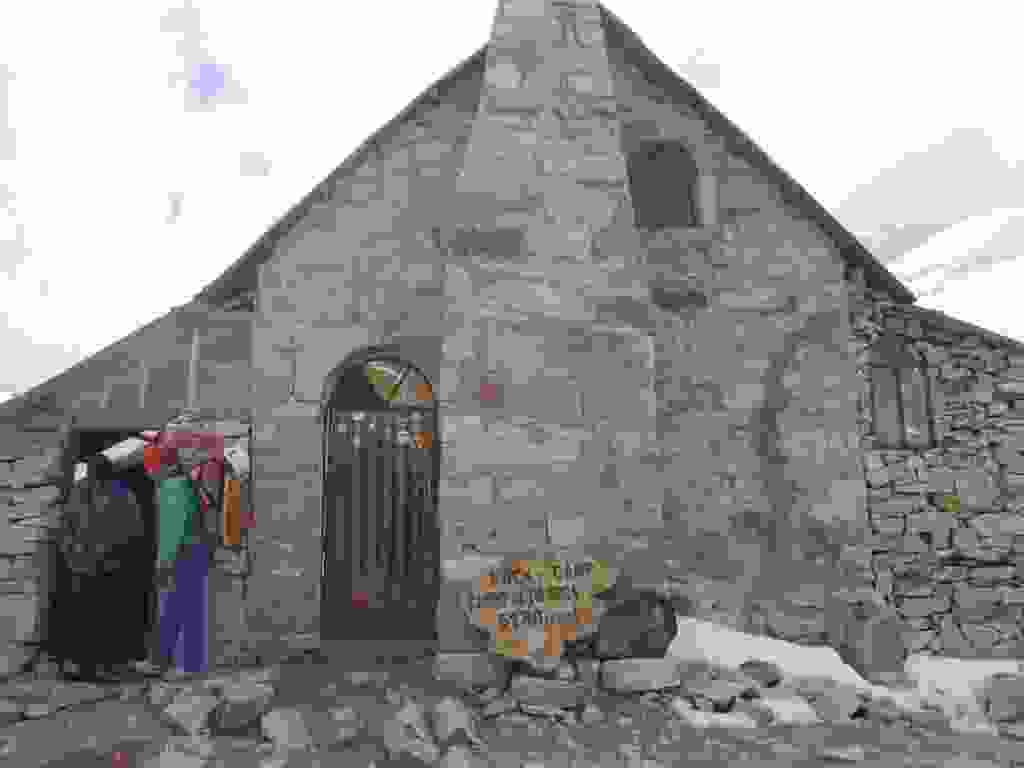
\includegraphics[width=\mywidth]{../wp-content/uploads/2015/05/P5013717-1024x768.jpg} \end{center}
\begin{center} 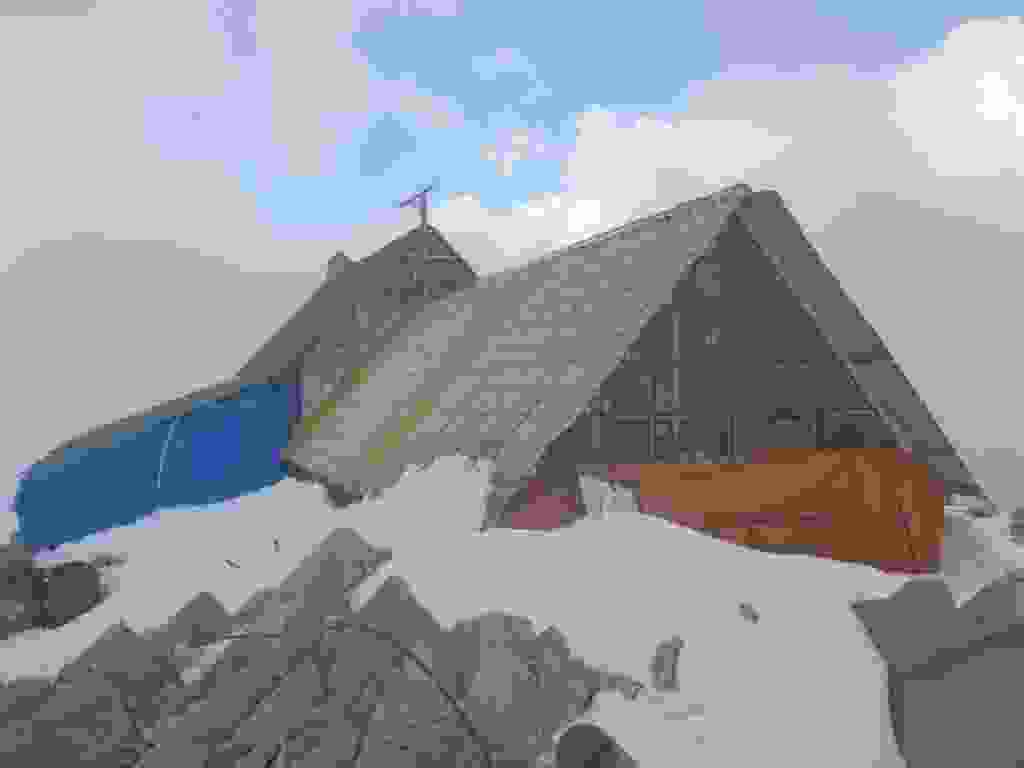
\includegraphics[width=\mywidth]{../wp-content/uploads/2015/05/P5013728-1024x768.jpg} \end{center}
\pagebreak

Dîner à 17h pour se lever le lendemain à minuit ! 
\begin{center} 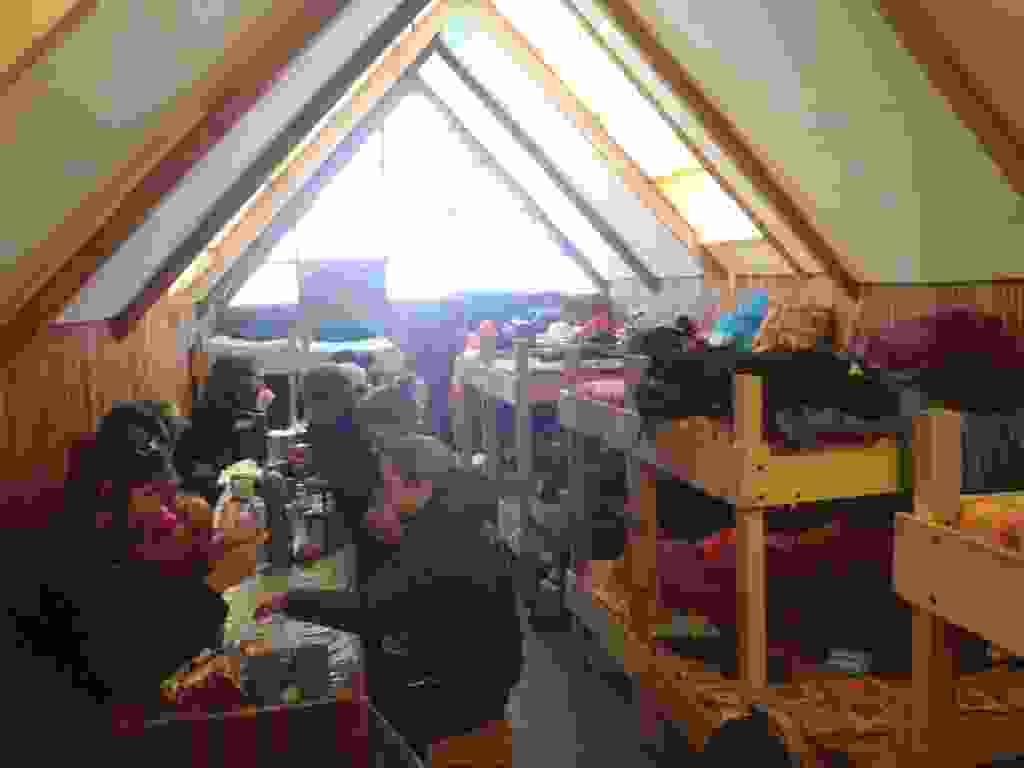
\includegraphics[width=\mywidth]{../wp-content/uploads/2015/05/P5013723-1024x768.jpg} \end{center}

L'ascension commence à 1h, encordé avec mon guide Sebastian. Au départ la Lune éclaire assez pour monter sans frontale. La montée est régulière sur la neige. Un seul passage est difficile : on doit s'aider du piolet pour monter. Enfin, la partie avant le sommet est délicate : très raide et en fort dévers. 

\begin{center} 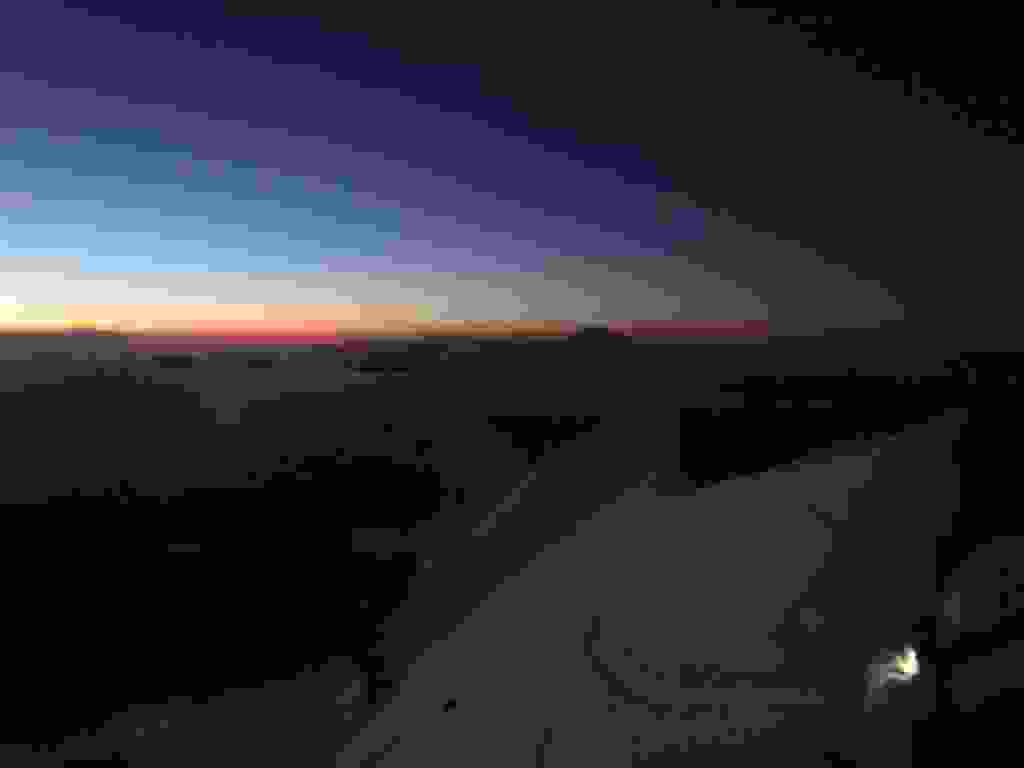
\includegraphics[width=\mywidth]{../wp-content/uploads/2015/05/P5023739-1024x768.jpg} \end{center}
\pagebreak

Vers 6h on arrive au sommet à 6088m, le jour n'est même pas levé. L'ascension était physique mais je n'ai pas été trop gêné par l'altitude, je n'ai pas trop perdu l'acclimatation des 12 jours dans le Sud Lipez. 
\begin{center} 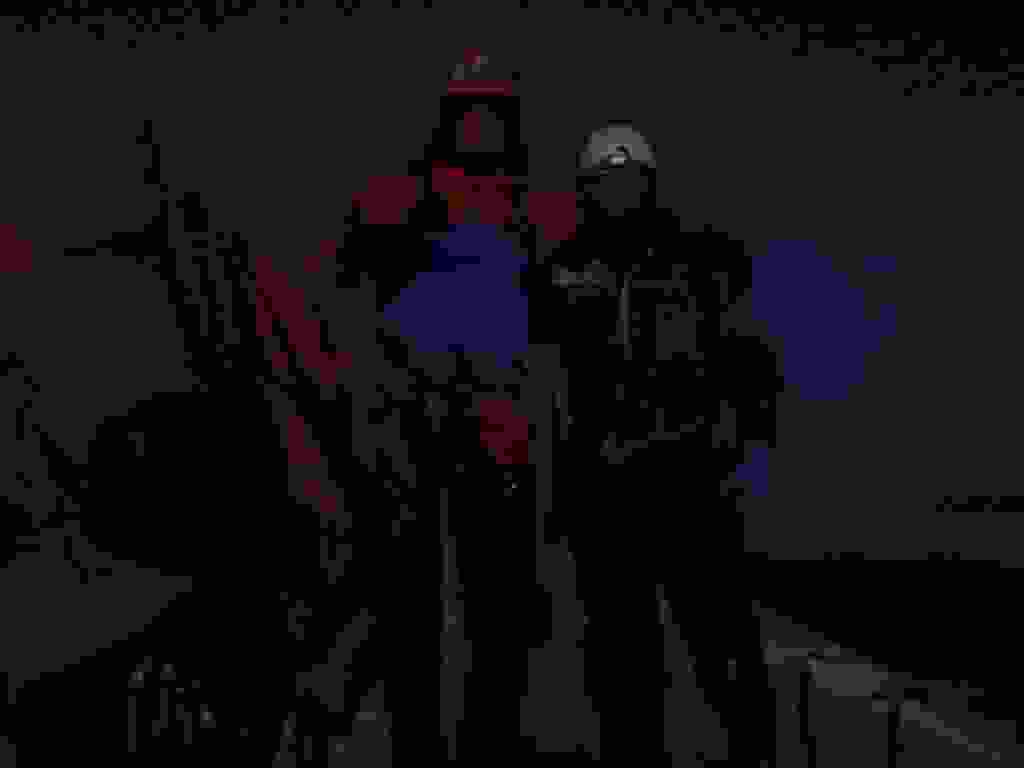
\includegraphics[width=\mywidth]{../wp-content/uploads/2015/05/P5023742-1024x768.jpg} \end{center}
\begin{center} 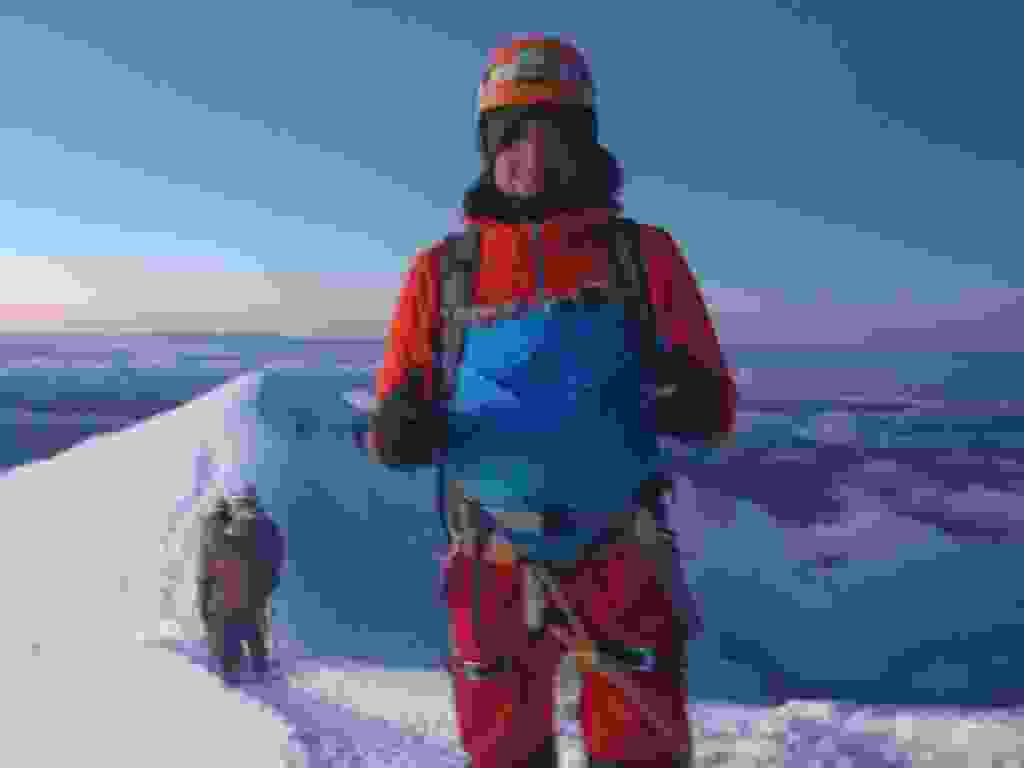
\includegraphics[width=\mywidth]{../wp-content/uploads/2015/05/P5023745-1024x768.jpg} \end{center}

\begin{center} 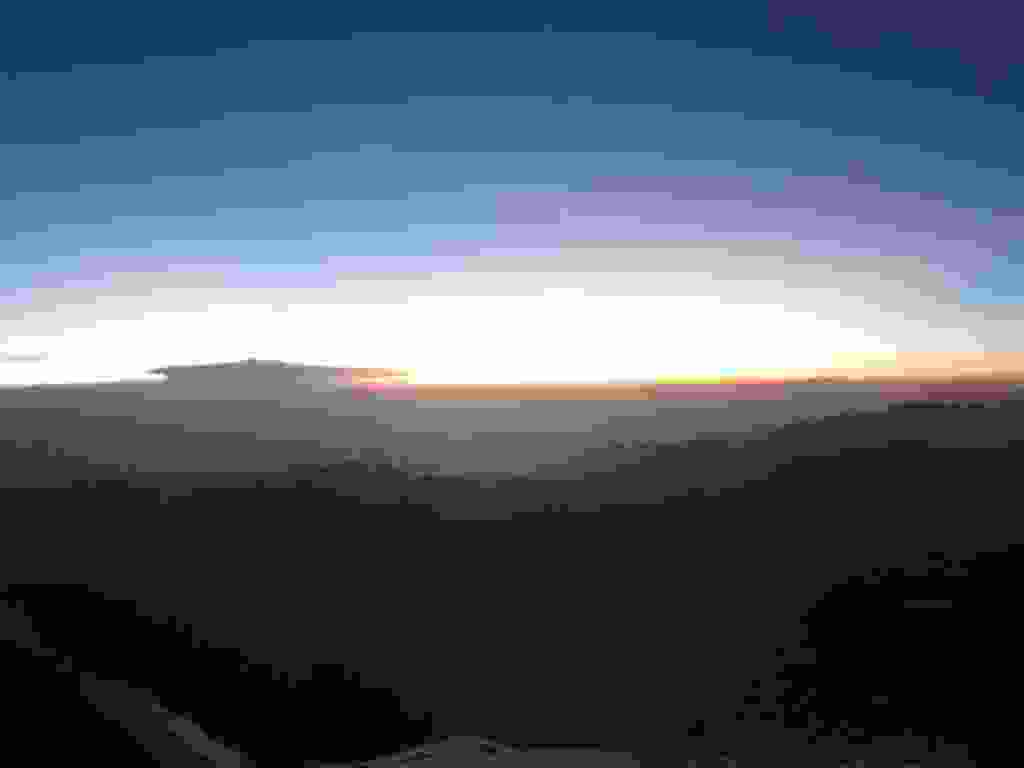
\includegraphics[width=\mywidth]{../wp-content/uploads/2015/05/P5023744-1024x768.jpg} \end{center}

Puis descente sous un magnifique soleil, à 11h on est de retour au camp de base. 
\begin{center} 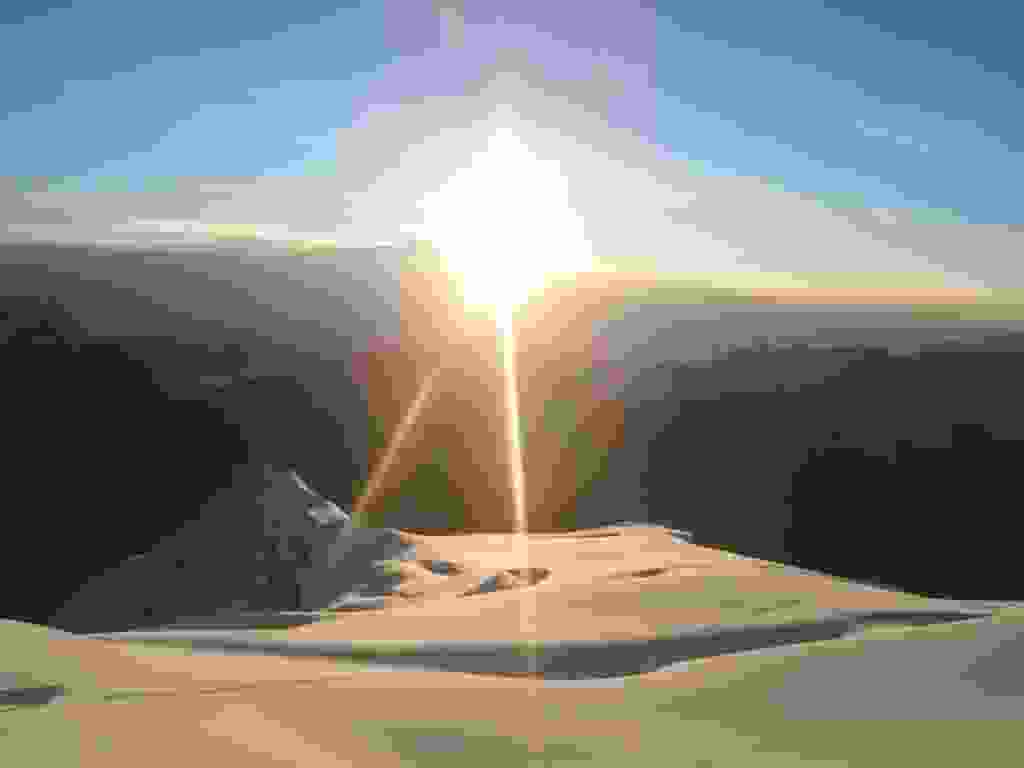
\includegraphics[width=\mywidth]{../wp-content/uploads/2015/05/P5023747-1024x768.jpg} \end{center}

\begin{center} 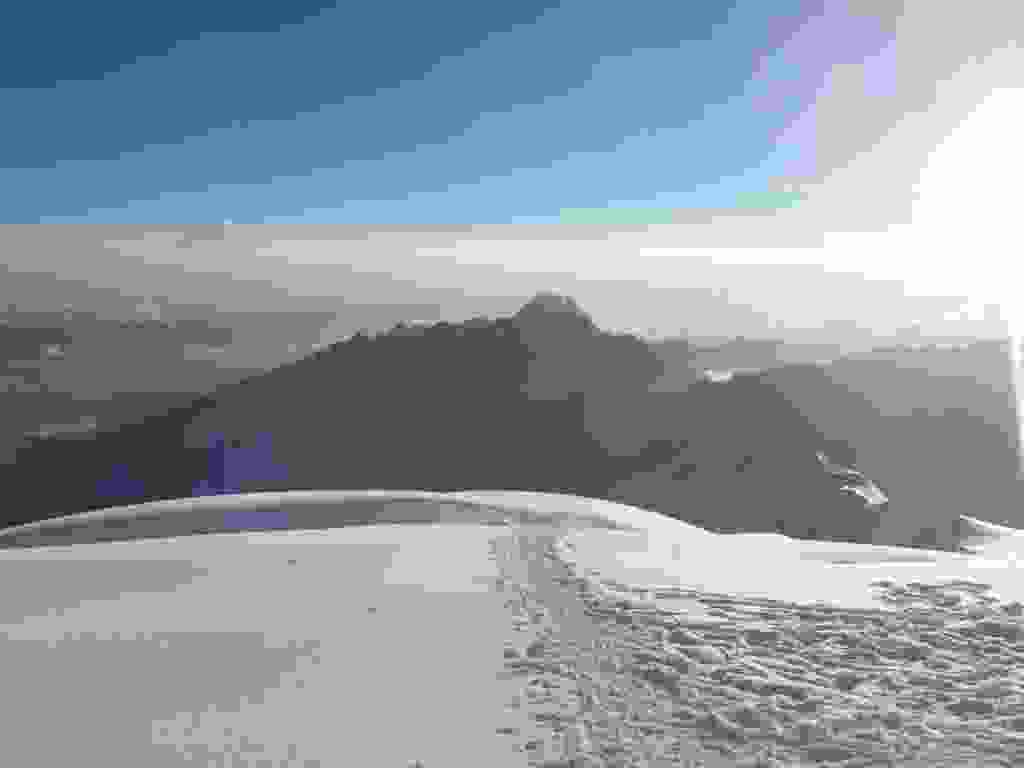
\includegraphics[width=\mywidth]{../wp-content/uploads/2015/05/P5023749-1024x768.jpg} \end{center}
\begin{center} 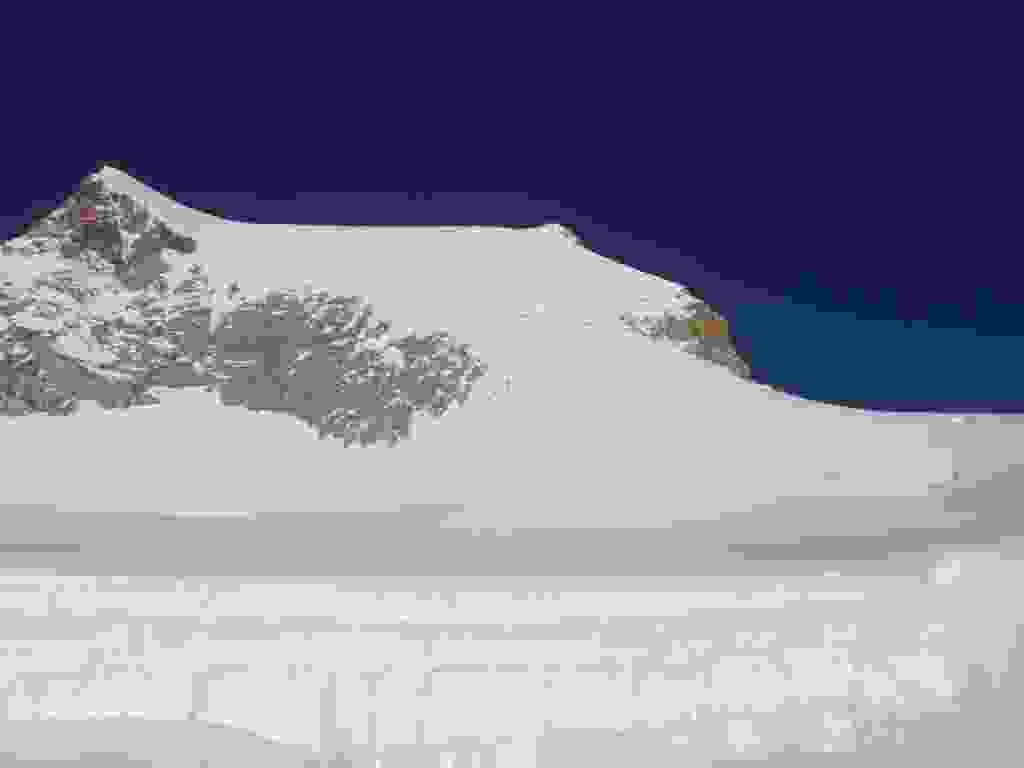
\includegraphics[width=\mywidth]{../wp-content/uploads/2015/05/P5023751-1024x768.jpg} \end{center}

\begin{center} 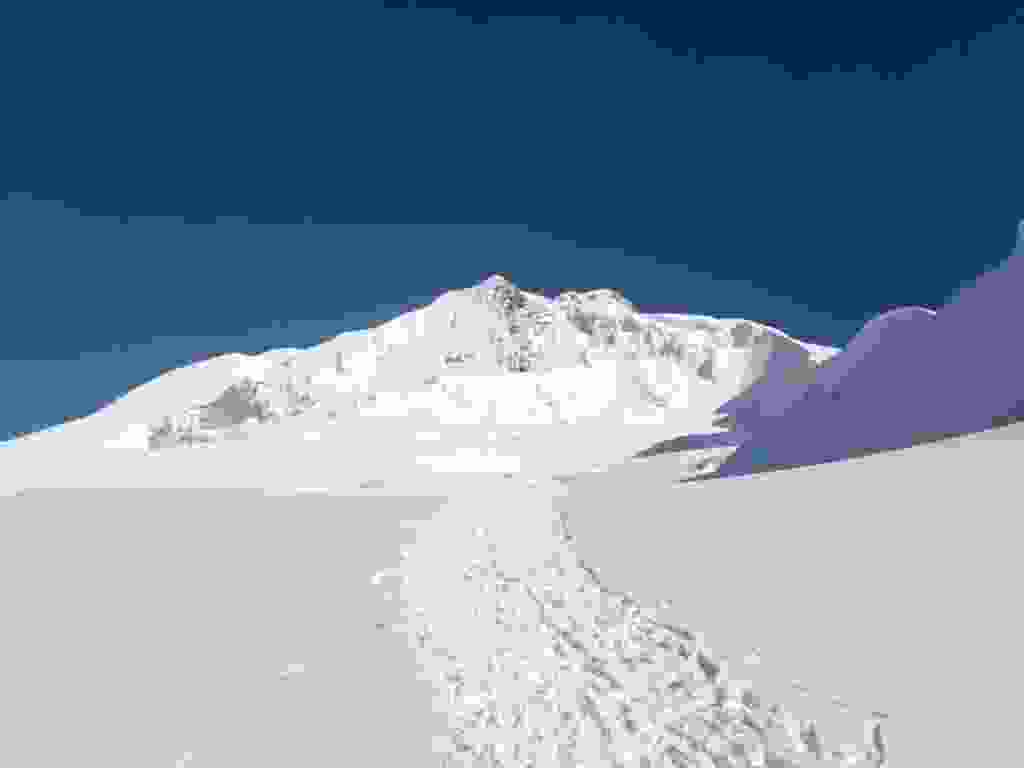
\includegraphics[width=\mywidth]{../wp-content/uploads/2015/05/P5023755-1024x768.jpg} \end{center}
\begin{center} 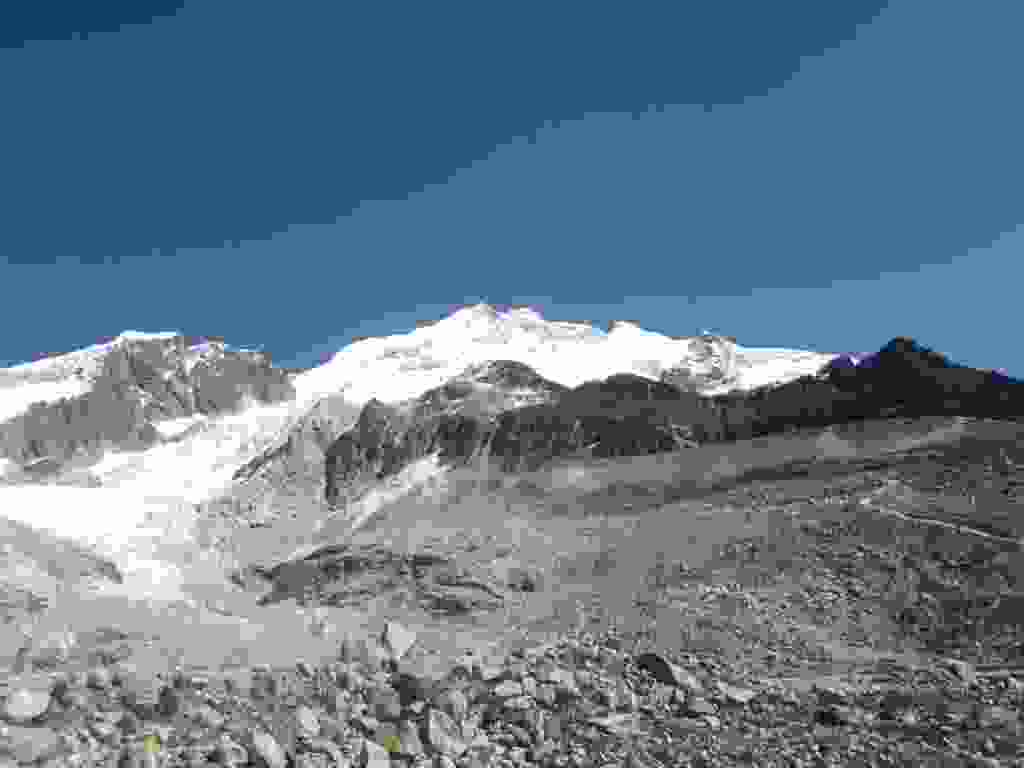
\includegraphics[width=\mywidth]{../wp-content/uploads/2015/05/P5023756-1024x768.jpg} \end{center}
\pagebreak

À côté de La Paz se trouve aussi la fameuse route de la mort qui serpente à flan de montagne sur 70km vers la région des Yungas. Je suis allé faire la descente en VTT avec un tour organisé. On monte en minibus au départ de la route à 4650m. Les 20 premiers km sont sur du bitume. 
\begin{center} 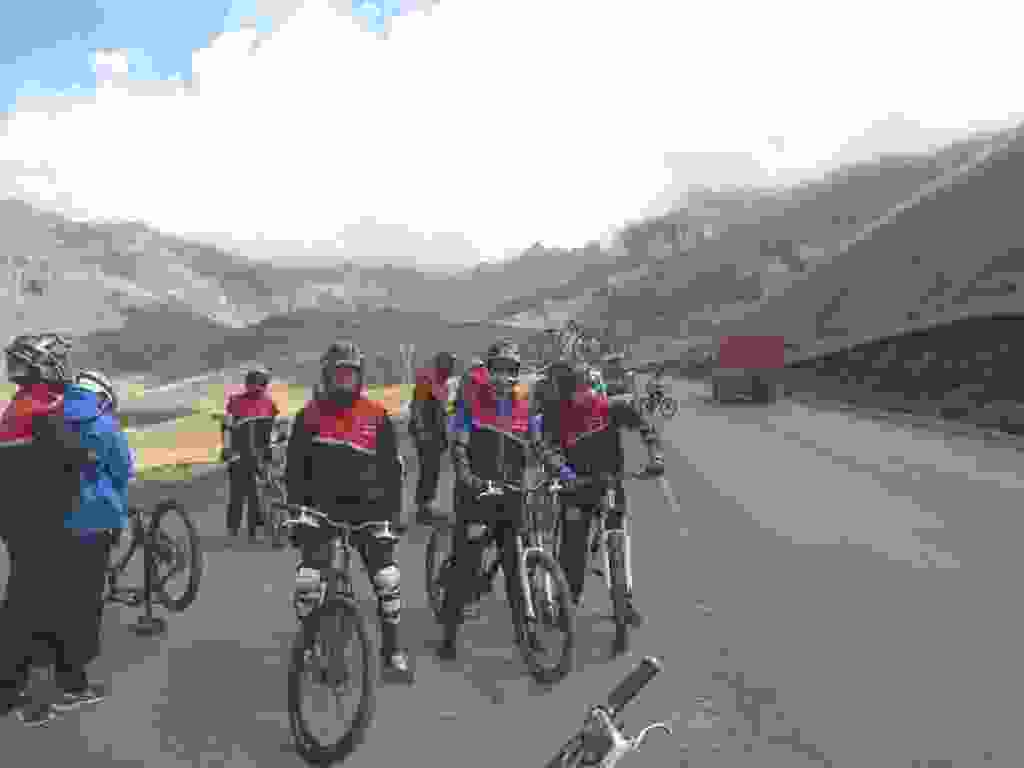
\includegraphics[width=\mywidth]{../wp-content/uploads/2015/05/P5043759-1024x768.jpg} \end{center}

Puis la vraie route de la mort commence : la seule route de Bolivie où l'on roule à gauche, savez-vous pourquoi ? 
\begin{center} 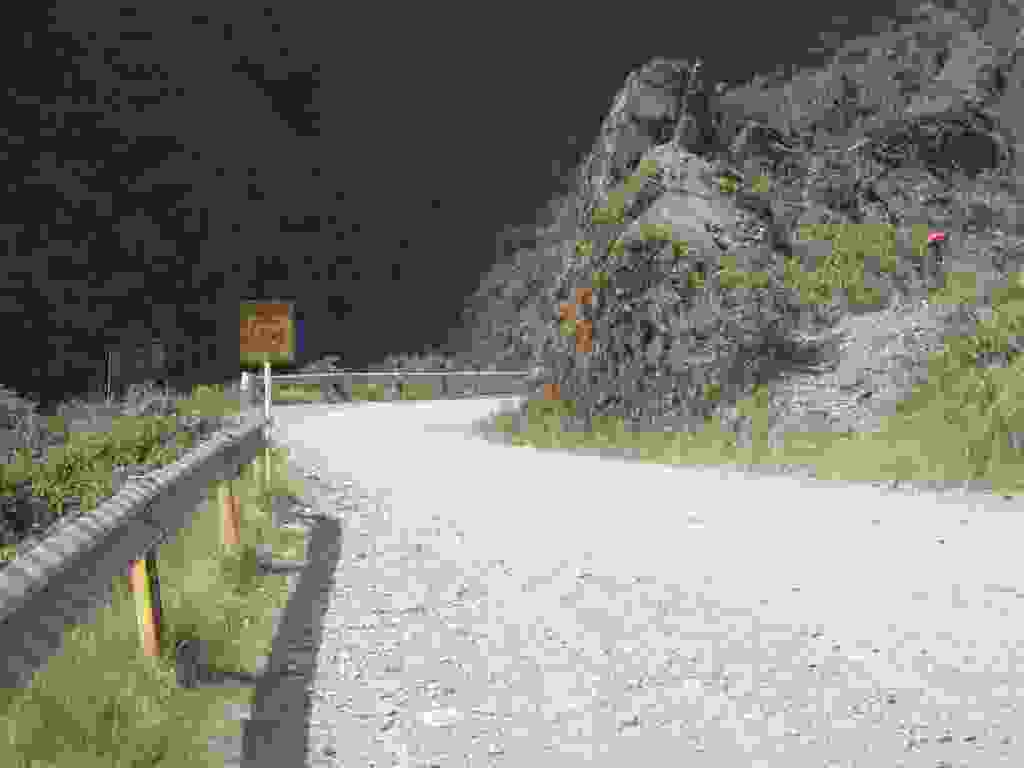
\includegraphics[width=\mywidth]{../wp-content/uploads/2015/05/P5043761-1024x768.jpg} \end{center}

\begin{center} 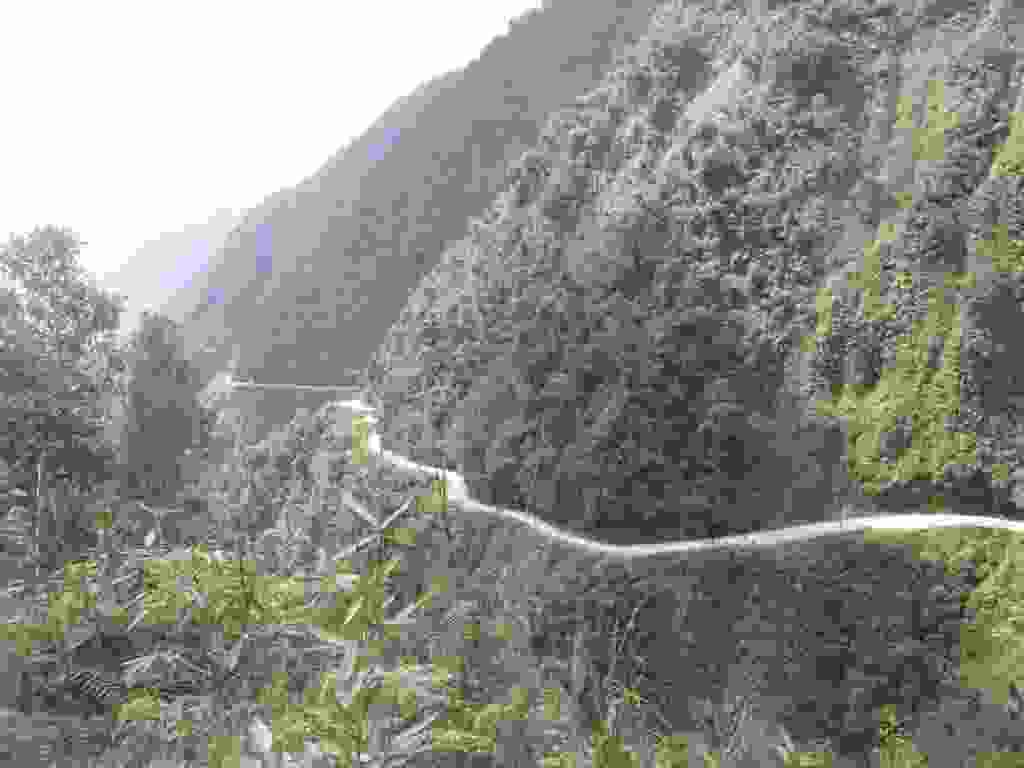
\includegraphics[width=\mywidth]{../wp-content/uploads/2015/05/P5043766-1024x768.jpg} \end{center}
\begin{center} 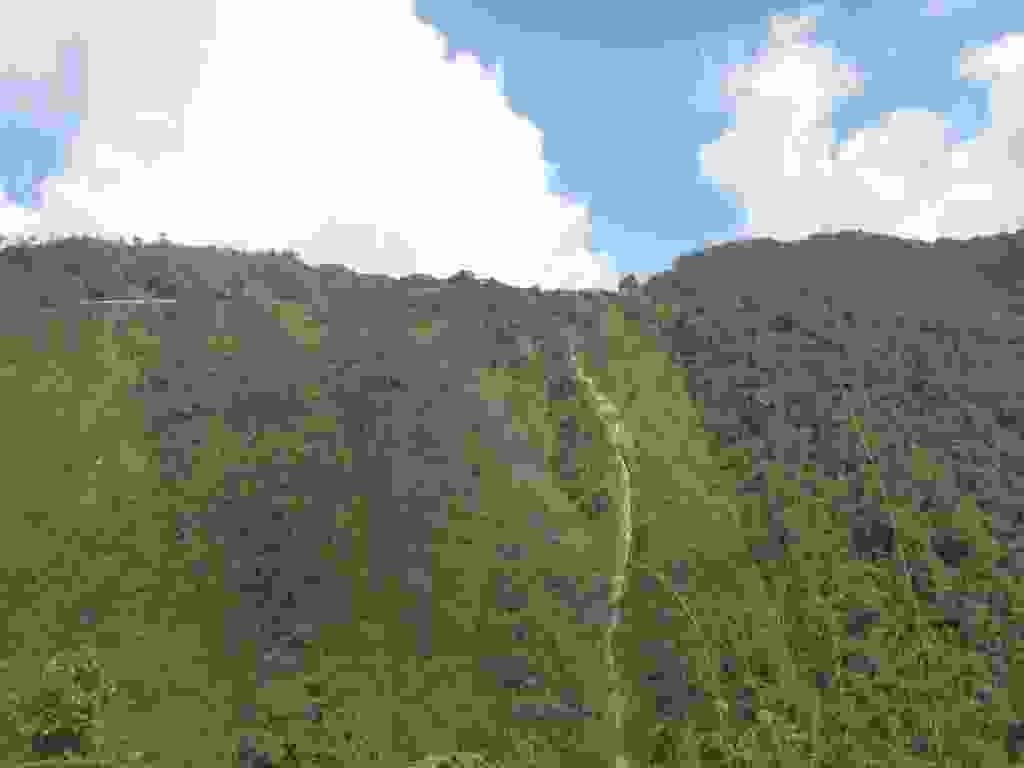
\includegraphics[width=\mywidth]{../wp-content/uploads/2015/05/P5043763-1024x768.jpg} \end{center}
\pagebreak

La végétation est luxuriante et la température monte rapidement au fur et à mesure. 
\begin{center} 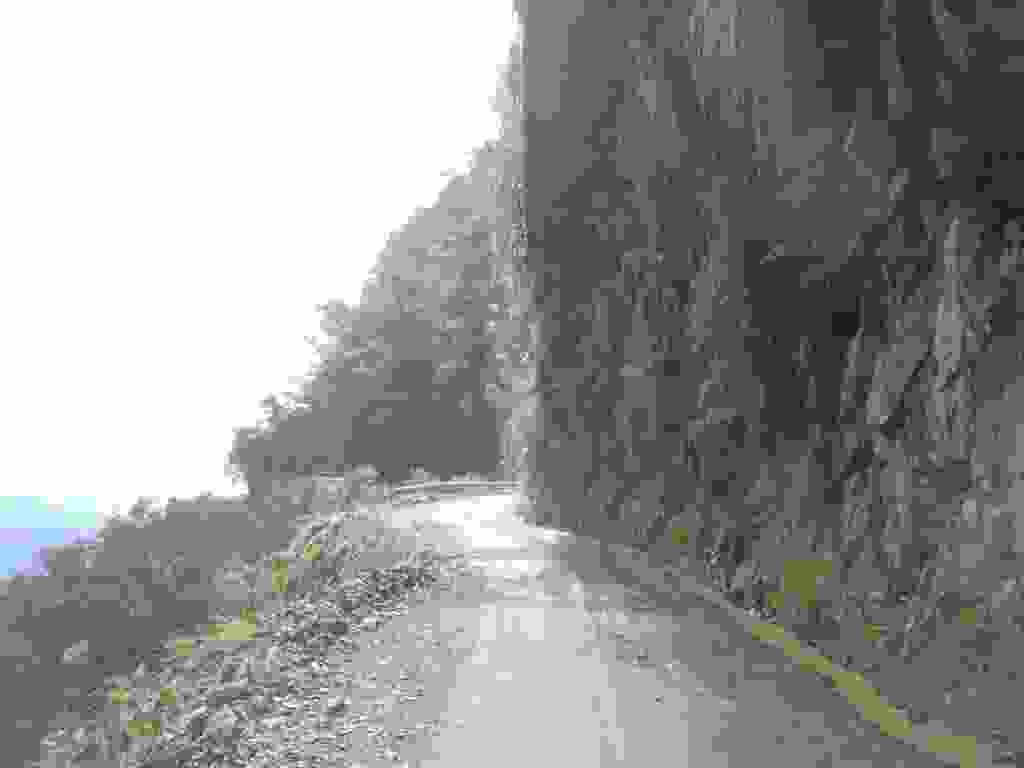
\includegraphics[width=\mywidth]{../wp-content/uploads/2015/05/P5043765-1024x768.jpg} \end{center}
\begin{center} 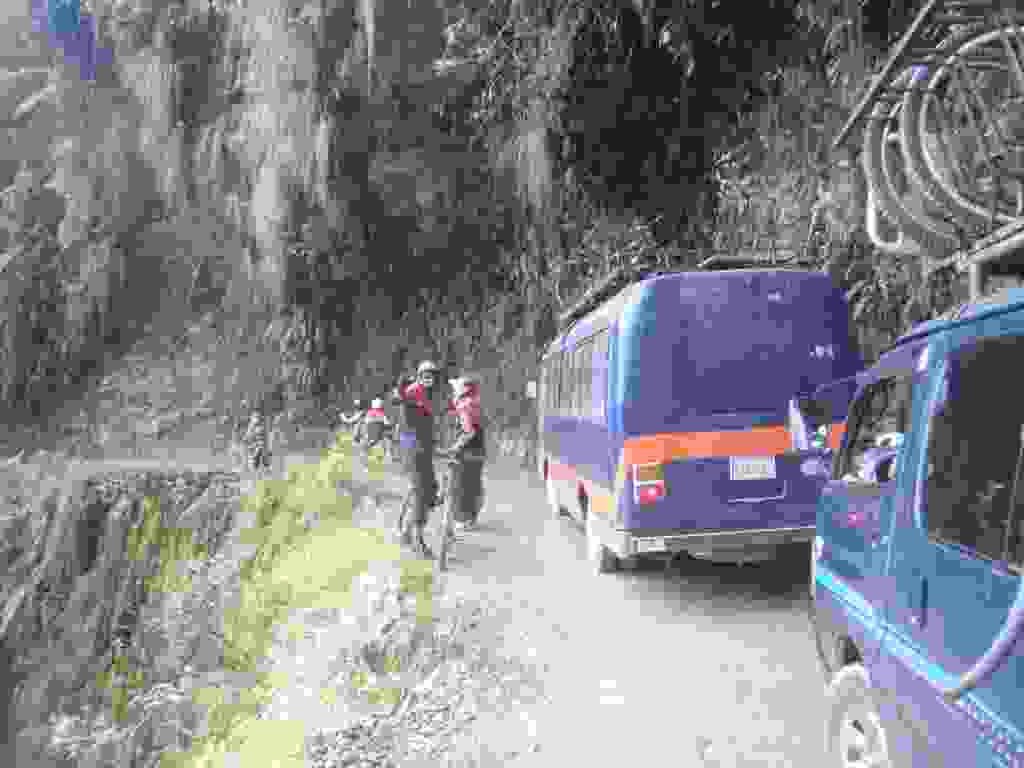
\includegraphics[width=\mywidth]{../wp-content/uploads/2015/05/P5043771-1024x768.jpg} \end{center}

\begin{center} 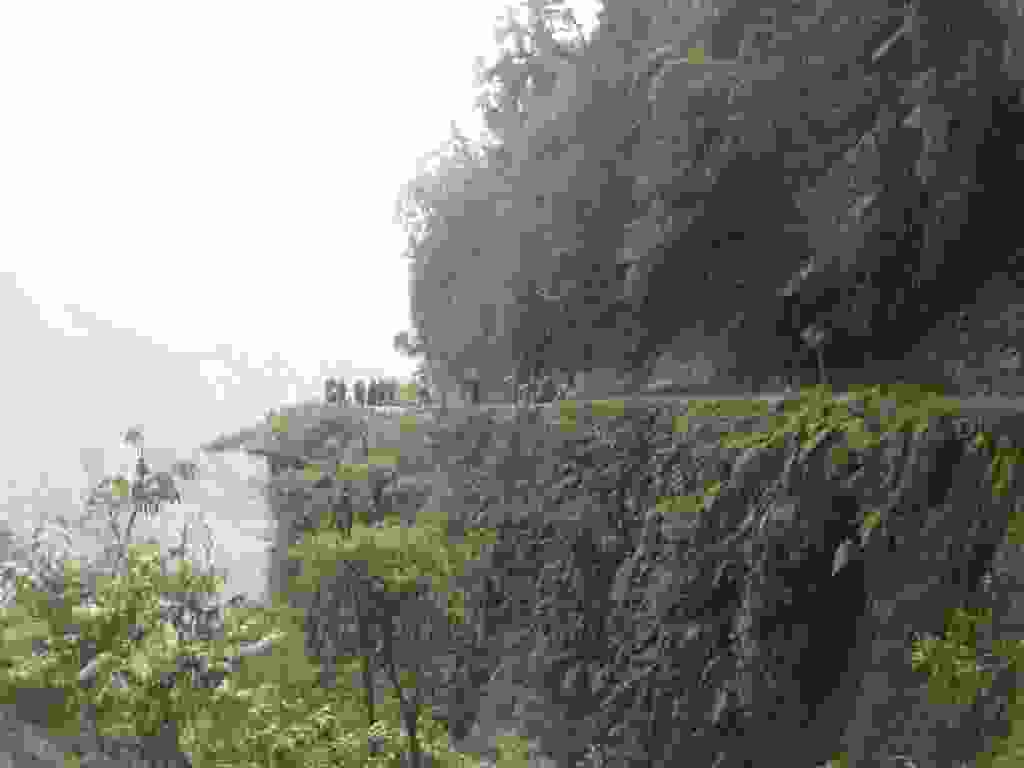
\includegraphics[width=\mywidth]{../wp-content/uploads/2015/05/P5043770-1024x768.jpg} \end{center}
\begin{center} 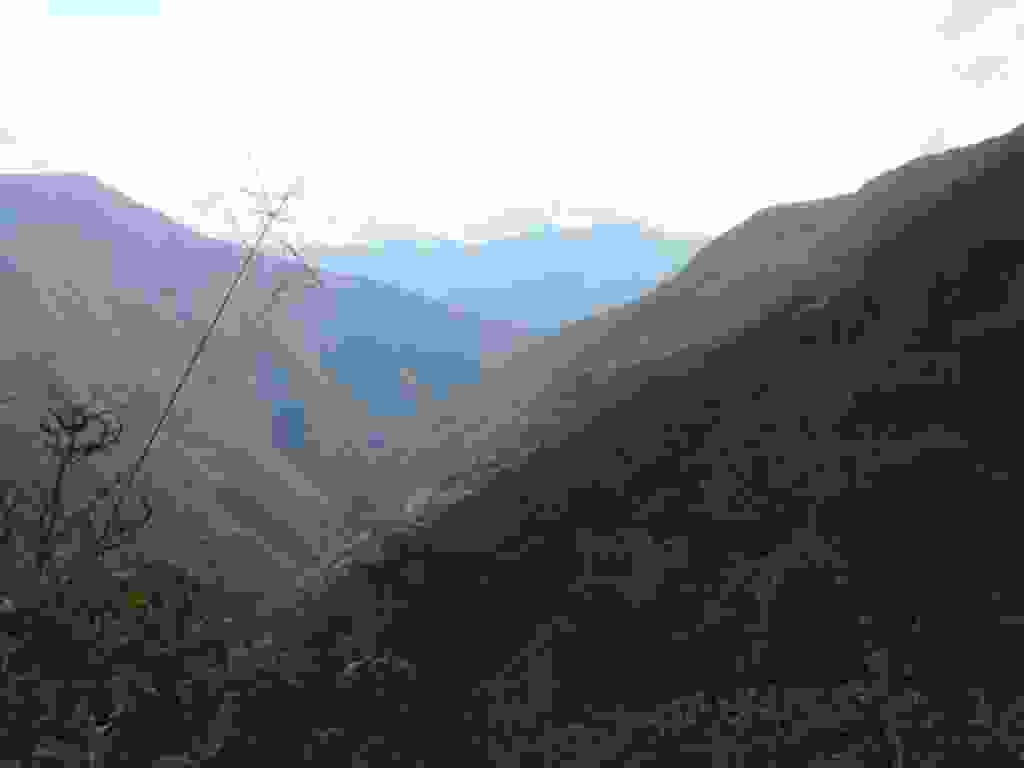
\includegraphics[width=\mywidth]{../wp-content/uploads/2015/05/P5043777-1024x768.jpg} \end{center}
\pagebreak

La route finit quasiment dans la jungle à 1200m d'altitude. 
\begin{center} 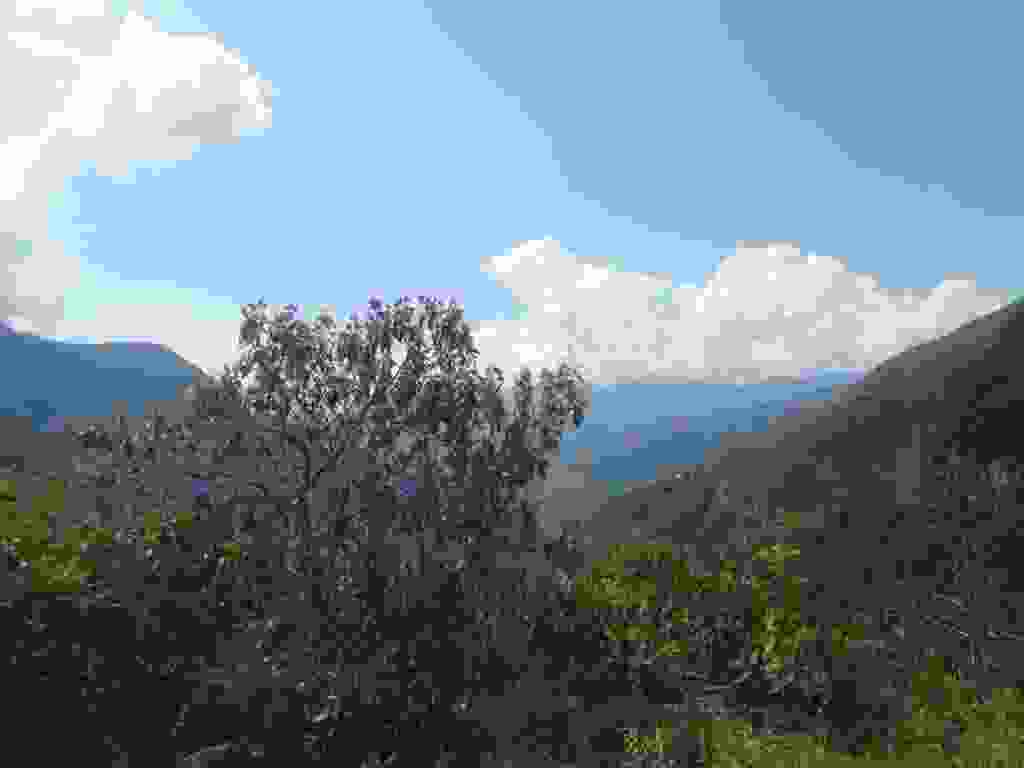
\includegraphics[width=0.8\textwidth]{../wp-content/uploads/2015/05/P5043784-1024x768.jpg} \end{center}

Aujourd'hui ça n'est plus vraiment une route de la mort, elle a été remplacée par une autre route toute asphaltée. Du coup il y a très peu de trafic. Un peu de repos à la casa de ciclistas et je continue vers le nord. Je sors de la ville en compagnie de 2 cyclistes suisses, Sonia et Gabriel.

La sortie de La Paz : 12.5km de montée et une vingtaine de km dans les gaz d'échappement. 
\begin{center} 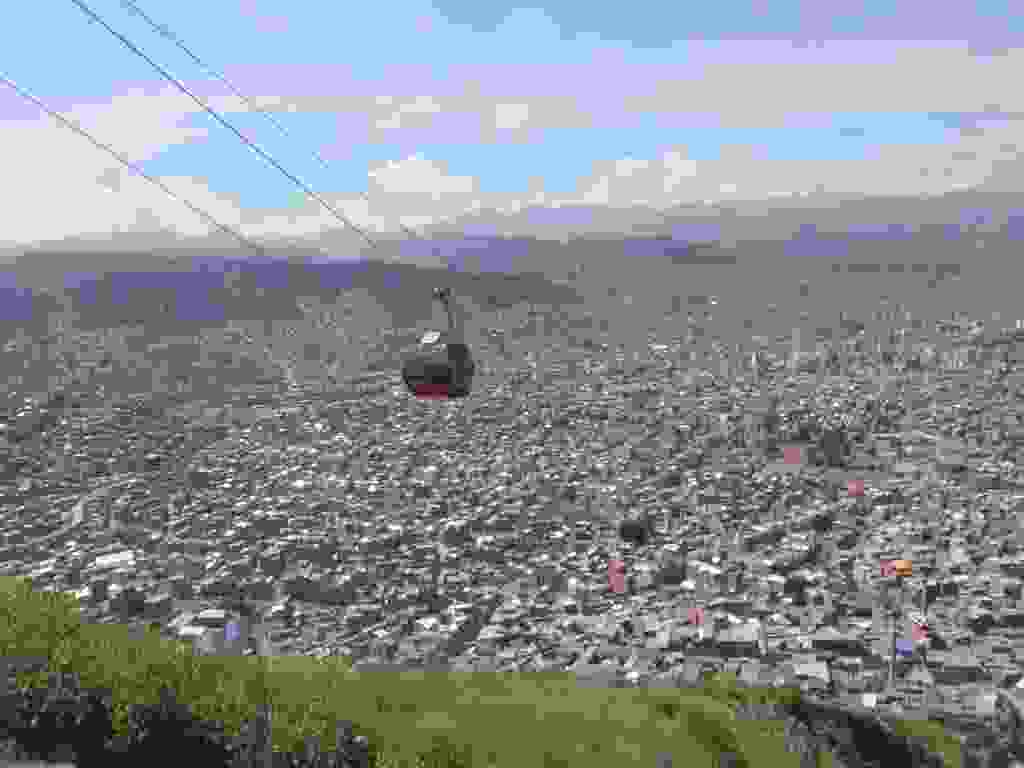
\includegraphics[width=0.8\textwidth]{../wp-content/uploads/2015/05/P5053792-1024x768.jpg} \end{center}

\begin{center} 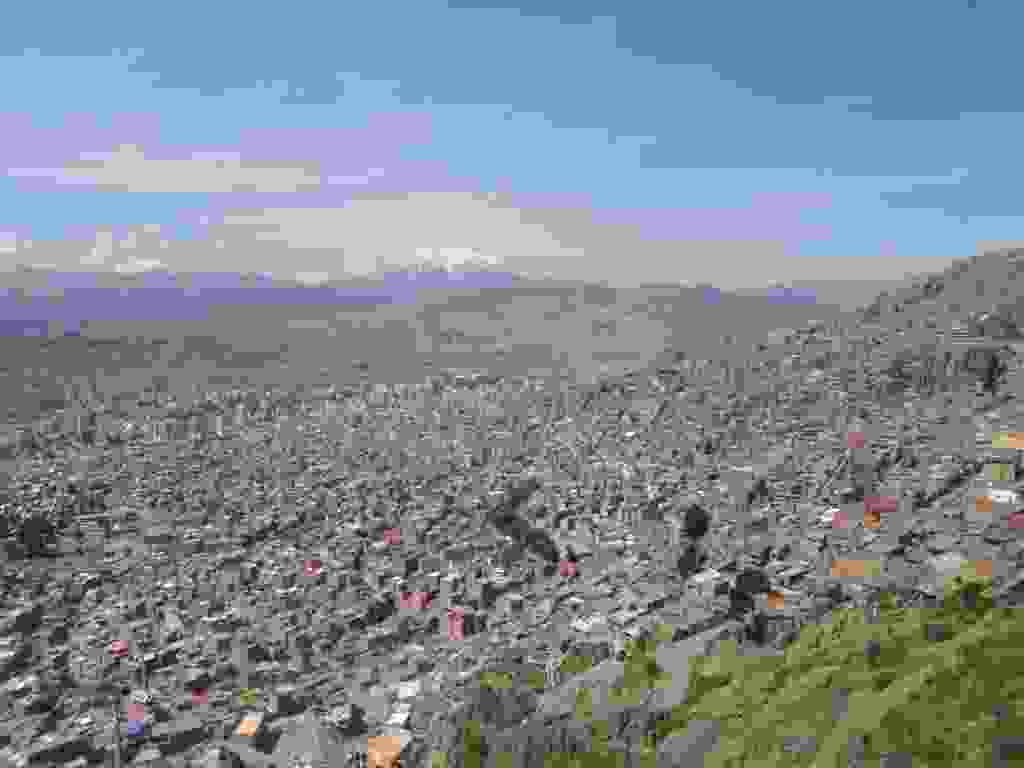
\includegraphics[width=\mywidth]{../wp-content/uploads/2015/05/P5053793-1024x768.jpg} \end{center}
\begin{center} 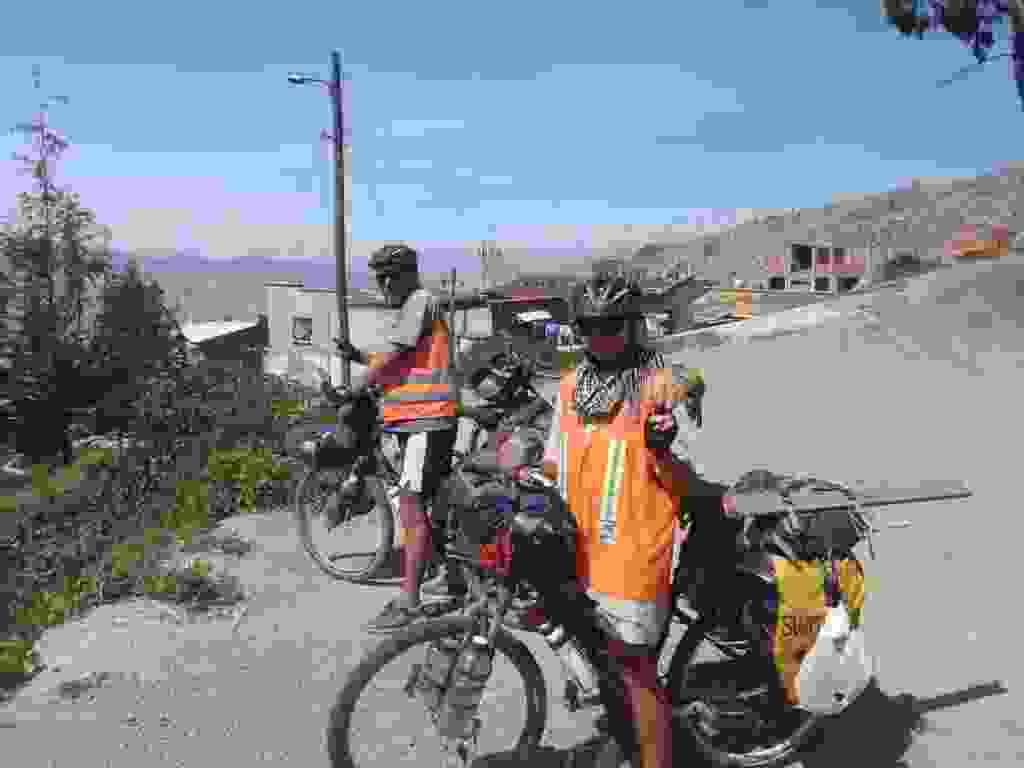
\includegraphics[width=\mywidth]{../wp-content/uploads/2015/05/P5053791-1024x768.jpg} \end{center}

\begin{center} 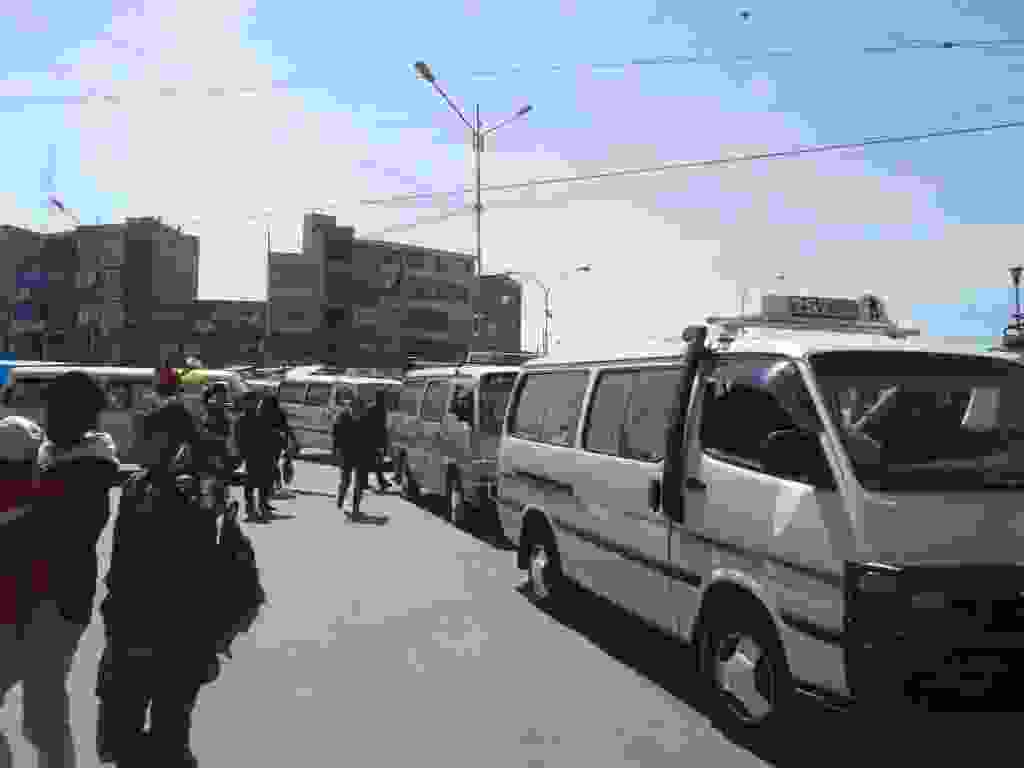
\includegraphics[width=\mywidth]{../wp-content/uploads/2015/05/P5053795-1024x768.jpg} \end{center}
